\documentclass[10pt,a4paper]{article}

\usepackage[a4paper,margin=20mm]{geometry}
\usepackage[T1]{fontenc}
\usepackage{mathptmx}
\usepackage{float}
\usepackage[scaled=.92]{helvet}
\usepackage{courier}
\usepackage{amsmath,amssymb,mathtools}
\usepackage{graphicx}
\usepackage{booktabs}
\usepackage{tabularx}
\usepackage{caption}
\usepackage{xcolor}
\usepackage{fancyhdr}
\usepackage[expansion=false]{microtype}
\usepackage[hidelinks]{hyperref}

\definecolor{primary}{RGB}{13,27,42}
\definecolor{accent}{RGB}{217,93,36}
\definecolor{teal}{RGB}{15,110,140}
\definecolor{muted}{RGB}{82,96,114}

\hypersetup{
  colorlinks=true,
  linkcolor=primary,
  citecolor=teal,
  urlcolor=teal,
  pdftitle={Apex-Continuum-50 v2: Zero-Trust Continuum Verification of a 50 MW Thermal-to-sCO2 Long-Duration Energy Storage Plant},
  pdfauthor={Bruce McGinley}
}

\setlength{\parskip}{5.5pt plus 2pt minus 1pt}
\setlength{\parindent}{0pt}
\captionsetup{font=small,labelfont={bf,color=primary}}

\pagestyle{fancy}
\fancyhf{}
\fancyhead[L]{\footnotesize\color{muted}\textsc{Apex-Continuum-50 v2 --- Scientific Proof-of-Concept Paper}}
\fancyhead[R]{\footnotesize\color{muted}\textsc{Zero-Trust Continuum Audited Baseline}}
\fancyfoot[C]{\footnotesize\color{muted}\thepage}
\renewcommand{\headrulewidth}{0.4pt}
\renewcommand{\footrulewidth}{0pt}

\setlength{\headheight}{14pt}
\setlength{\emergencystretch}{2em}
\begin{document}

% --- Title Block ---

\begin{center}
  {\small\bfseries\color{teal}\textsc{Scientific proof of concept \enspace | \enspace 25 November 2026}}\\[12pt]
  {\Huge\bfseries\color{primary} Apex-Continuum-50 v2}\\[8pt]
  {\Large\color{primary} Continuum Verification of a 50 MW Thermal-to-sCO\textsubscript{2} Storage Plant}\\[8pt]
  {\small\color{muted} Bruce McGinley \quad$\cdot$\quad Open-Source Release (CC-BY-4.0 / CERN-OHL-P v2 / MIT)}
\end{center}
\vspace{8pt}
\textbf{Abstract.}
Apex-Continuum-50 v2 couples a zero-salt magnesia-spinel thermal store to a dry-cooled, reheat supercritical CO\textsubscript{2} recompression Brayton cycle. A sequential CalculiX, OpenFOAM, and CoolProp audit determined which component results could carry into the plant model. The conformal 740H surge model yielded 112.60\,MPa peak bond-node von Mises stress with 1.15\% finest-mesh drift. The rectified \texttt{HDR\_F9} delivered 6.22\,kPa header-only loss with 6.92\% maximum port deviation. \texttt{RIB\_F8} was excluded after slightly lower heat transfer and 14.25\% higher upper-window friction than the archived control. A 192-interval real-gas closure estimates 50.00\,MW net AC and 52.36\% AC round-trip efficiency at 20\,\textdegree C, falling to 45.08\,MW and 48.49\% at 42\,\textdegree C. With full Inconel 740H and \$65.50M in modeled block CAPEX, the corresponding 24/100\,h LCOS is \$82.48/\$98.50 per MWh at ISO and \$89.86/\$107.05 per MWh in summer.
\vspace{4pt}

% --- Section 1 ---

\section{Introduction}

In a thermal storage plant, the refractory inventory determines energy capacity and the power block determines electrical output. The Apex architecture uses that separation to study 24- and 100-hour duration on the same 50\,MW power block. Its conversion path builds on supercritical CO\textsubscript{2} pilot work such as the U.S. Department of Energy and GTI Energy STEP program \cite{step_demo}. At this stage, recuperator metallurgy, header hydraulics, and film heat transfer are material drivers of the plant calculation.

The study takes the campaign design as a set of hypotheses. It retains the 740H recuperators after comparing stress and temperature evidence, carries the rectified header loss into the cycle, and uses the archived Variant B pin-rib result after the thermal/hydraulic gate rejected the candidate. The economic reconciliation shows the effect of those choices at both ambient points and both storage durations.

\subsection*{Evidence convention}
\begin{tabularx}{\linewidth}{@{}lX@{}}
\toprule
\textbf{Class} & \textbf{Scope in this paper}\\
\midrule
\textsf{MEASURED} & Numerical quantities reduced from saved CalculiX or OpenFOAM solutions. Reported pressures and stresses depend on the documented load, boundary conditions, mesh, and sampling window.\\
\textsf{MODELED} & Thermodynamic output, RTE, component cost assumptions, LCOS, and parametric CAD. The whole-plant figures use the 192-interval HEOS closure and the cost model.\\
\textsf{HARDWARE} & Open experimental and procurement gates in Section~\ref{sec:limits}.\\
\bottomrule
\end{tabularx}

\medskip
The frozen claim ledger, result links, and solver commands reside in the final audit report \cite{audit}. Figures~\ref{fig:fea3d} and \ref{fig:hdr3d} use the corresponding archived field data. Figure~\ref{fig:architecture3d} uses the handoff CAD at its native dimensions.

\clearpage
% --- Section 2 ---
\section{System Architecture and Zero-Trust Verification Protocol}


\subsection{TS\_F10 thermal battery and dry power block}
The modeled store uses magnesia-spinel refractory with a 6:1 slit-opening geometry and an external Kanthal/SiC charging plenum. Figure~\ref{fig:architecture3d} shows a representative stack section and the plant arrangement. The thermal storage inputs are \$8.99/kWh\textsubscript{th} and a 0.991 combined charge and thermal factor. The concept places six vaults and external plenums beside the sCO\textsubscript{2} hall and four dry-cooler bays on a 90\,m by 65\,m pad.

The reheat RCBC retains the 0.95\,m Variant B LTR, Inconel 740H PCHEs, and independent 0.39 ISO / 0.34 summer recompression splits. The modeled geared 3,600\,RPM generator uses 97.86\% conversion and \$151 per gross kW\textsubscript{e}, with a \$200,000 control hardware allowance.

\begin{figure}[H]
  \centering
  \includegraphics[width=.485\linewidth]{render_3d_plant_pad.png}\hfill
  \includegraphics[width=.485\linewidth]{render_3d_tsf10_brick.png}
  \caption{\textsf{MODELED} parametric architecture, with orthographic scale bars. The plant layout identifies the six vaults and dry-cooling bays. The stack section shows 36\,mm by 6\,mm slit openings and the 120\,mm microporous insulation envelope. The two panels use independent physical scales.}
  \label{fig:architecture3d}
\end{figure}

\subsection{Computational method}

Cycle closure solves the 192-interval real-gas enthalpy balance across both LTR and high-temperature recuperator (HTR) using \texttt{CoolProp 7.2.0} \texttt{HEOS::CO2} \cite{coolprop_api}, enforcing positive minimum pinch $\Delta T_{\min}$ across all sub-intervals $k \in \{1,\dots,192\}$:
\begin{equation}
  \dot{m}_h \bigl(h_{h,k} - h_{h,k-1}\bigr) = \dot{m}_c \bigl(h_{c,k} - h_{c,k-1}\bigr) = (UA)_k\,\Delta T_{\text{lm},k}, \qquad \min_{k} \bigl(T_{h,k} - T_{c,k}\bigr) > 0.
  \label{eq:pinch}
\end{equation}

The header model applies the OpenFOAM \texttt{porousBafflePressure} jump condition \cite{of_baffle}. The archived Option A Variant B HTR response supplies film $Nu = 43.66$ ($0.5942$ times the analytic reference) and upper-window $f = 0.01160$ ($0.96053$ times the analytic reference).

Electricity-only LCOS follows the locked financial convention ($r_{\text{CRF}} = 8.02\%$, charging price $P_{\text{chg}} = \$25/\text{MWh}$, $N_{\text{cyc}} = 180\,\text{yr}^{-1}$ at 24\,h and $50\,\text{yr}^{-1}$ at 100\,h):
\begin{equation}
  \text{LCOS} = \frac{r_{\text{CRF}}\cdot C_{\text{total}} + C_{\text{O\&M}}}{N_{\text{cyc}}\,E_{\text{net,AC}}} + \frac{P_{\text{chg}}}{\eta_{\text{AC,RTE}}}.
  \label{eq:lcos}
\end{equation}


The WSL2 audit ran under a 2.5\,GB systemd memory cap with swap disabled for each solver scope. The archived run and post-processing commands are listed in the audit report.

\clearpage
% --- Section 3 ---
\section{Gate 1: CalculiX 3D Conformal Surge FEA and Metallurgy Rectification}

Campaign II proposed replacing ASME Code Case 2702 Inconel 740H \cite{inconel740h} in the 0.95\,m LTR with ASME SA-240 Duplex 2205 ($E = 190\,\text{GPa}$, $\nu = 0.30$, screening limit 175\,MPa at 240\,\textdegree C) to save \$6.58M. Gate 1 tested three candidate alloys on the conformal Variant B LTR unit cell under 440.25\,bar high-pressure / 79\,bar low-pressure surge loading (+10\% etch screen, ideal bonded interfaces, constrained axial/lateral strain) across three mesh refinements (0.340, 0.270, and 0.220\,mm target element sizes via Gmsh 4.12.1 \texttt{libgmsh.so.4.12.1}).

\begin{table}[H]
  \centering
  \caption{Gate 1 CalculiX C3D10 conformal surge FEA results across three mesh levels (440.25\,bar / 79\,bar).}
  \label{tab:gate1}
  \footnotesize\setlength{\tabcolsep}{3.5pt}
  \begin{tabularx}{\linewidth}{l r c c r r r X}
    \toprule
    \textbf{Material} & \textbf{Temp.} & \textbf{C3D10 Elements} & \textbf{Bond-Node $\sigma_{\text{vM}}$} & \textbf{Fine Peak} & \textbf{Finest-2} & \textbf{Limit} & \textbf{Audit Disposition} \\
     & (\textdegree C) & (Coarse / Med / Fine) & (MPa) & (MPa) & \textbf{Drift} & (MPa) & \\
    \midrule
    Duplex 2205 & 240 & 15,010 / 26,642 / 48,548 & 97.45 / 113.91 / 112.60 & 131.95 & 1.15\% & 175 & Clears 240\,\textdegree C screen; hot inlet uncertified \\
    Thick.\ SS316L & 240 & 17,987 / 32,361 / 58,314 & 98.92 / 114.03 / 117.53 & 133.47 & 3.07\% & 115 & \textbf{FAIL} ($>115$\,MPa screen) \\
    Retained 740H & 275 & 15,010 / 26,642 / 48,548 & 97.45 / 113.91 / 112.60 & 131.95 & 1.15\% & --- & \textbf{PASS} mesh screen; retained material \\
    \bottomrule
  \end{tabularx}
\end{table}

Although Duplex 2205 cleared the isothermal 240\,\textdegree C elastic stress screen (112.60\,MPa vs.\ 175\,MPa, 1.15\% mesh drift) and thickened SS316L (3.05\,mm rib / 3.20\,mm plate) failed its 115\,MPa limit at 117.53\,MPa, the coupled summer heat balance revealed that the hottest LTR fluid terminal reaches \textbf{262.76\,\textdegree C}---exceeding the 240\,\textdegree C zone basis without a certified wall-temperature profile or dissimilar-metal diffusion-bond transition. Under zero-trust rules, \textbf{\$0 of the \$6.58M duplex credit was carried into the baseline}, and full Inconel 740H (112.60\,MPa at 275\,\textdegree C) was retained across both recuperators (Figures~\ref{fig:fea3d} and \ref{fig:gates}A).


\begin{figure}[H]
  \centering
  \includegraphics[width=.94\linewidth]{render_3d_gate1_740h_fea.png}
  \caption{\textsf{MEASURED} CalculiX nodal von Mises field from the 48,548-element 740H \texttt{bond.frd} and conformal \texttt{bond.inp}. The undeformed exterior and the $z=0$ bond-plane cut use the same stress scale. The named bond and global maxima come from the full nodal result. Load case: 440.25/79\,bar at 275\,\textdegree C.}
  \label{fig:fea3d}
\end{figure}

The summer temperature is a fluid terminal from the plant model. A coupled wall-temperature assessment and a qualified transition are required before crediting any duplex substitution.

\clearpage
% --- Section 4 ---
\section{OpenFOAM Hydraulic and Thermal Gates}

\subsection{Gate 2: Dual-Entry Perforated Baffle Header Rectification (\texttt{HDR\_F9})}

The 340\,mm $\times$ 850\,mm dual-entry header was modeled in OpenFOAM v2312 \texttt{pimpleFoam} on a 33,408-cell mesh with four axial baffle stations, three full-span curved turning vanes (3\,mm axial bow), four outlets, and a 20.5\,kPa nominal downstream core porous jump at the Variant B HTR inlet state (309.05\,kg/s, 484.27\,K, $\text{Co} < 0.8$, $\sim$6 residence times). Flux-weighted total pressure taps were placed 9.286\,mm upstream and 10\,mm downstream of the core interface to prevent shared-face pressure artifacts.

\begin{table}[H]
  \centering
  \caption{Gate 2 OpenFOAM \texttt{pimpleFoam} 3D header audit: original vs.\ rectified \texttt{HDR\_F9} baffle tapers.}
  \label{tab:gate2}
  \footnotesize\setlength{\tabcolsep}{3.5pt}
  \begin{tabularx}{\linewidth}{l c r r r r r X}
    \toprule
    \textbf{Case} & \textbf{Open-Area} & \textbf{Header $\Delta P$} & \textbf{Core $\Delta P$} & \textbf{Mass} & \textbf{Max Port} & \textbf{Full Spread} & \textbf{Disposition} \\
     & \textbf{Zones} & (kPa) & (kPa) & \textbf{Imbal.} & \textbf{Dev.} & / Mean & \\
    \midrule
    HDR\_F8 (Prior) & Uniform & 11.733 & --- & 0.00455\% & 8.900\% & --- & Prior fallback benchmark \\
    Original F9 & 34/44/44/34\% & 25.345 & 21.054 & $2.91\times10^{-6}$\% & 9.316\% & 18.632\% & \textbf{FAIL} ($>11.7$\,kPa \& $>8.90\%$) \\
    Rectified F9 & 62/64/64/62\% & \textbf{6.222} & 20.969 & $2.80\times10^{-6}$\% & \textbf{6.917\%} & 13.834\% & \textbf{PASS} loss \& fallback dist. \\
    \bottomrule
  \end{tabularx}
\end{table}

The campaign's claimed 34\%/44\% taper failed decisively at 25.35\,kPa header loss and 9.32\% port deviation. Rectifying the open-area taper to 62\%/64\%/64\%/62\% slashed header-only loss by \textbf{75.5\%} to \textbf{6.22\,kPa} (47.0\% below prior \texttt{HDR\_F8}'s 11.73\,kPa) while improving max port deviation to 6.92\% with $2.80\times10^{-6}$\% mass imbalance (Table~\ref{tab:gate2}, Figure~\ref{fig:gates}B). Because port deviation remains above the preferred 2.5\% stretch goal (the campaign's 0.8\% headline was not reproduced), further baffle tuning is logged in the open risk register.


\begin{figure}[H]
  \centering
  \includegraphics[width=.98\linewidth]{render_3d_gate2_hdrf9_cfd.png}
  \caption{Rectified \texttt{HDR\_F9}. \textbf{A, \textsf{MEASURED}} 33,408-cell OpenFOAM checkpoint at 0.758263\,s. Curves are seeded from the saved velocity field. The pressure section shows $\rho(p_{\mathrm{kin}}+|\mathbf u|^2/2)$ relative to solver gauge. The 6.22\,kPa header-only result is the archived time-window tap average. \textbf{B, \textsf{MODELED}} parametric STL cutaway with four baffle stations and three vanes. The CFD and CAD panels have independent scale bars and use different geometric representations.}
  \label{fig:hdr3d}
\end{figure}

\clearpage
\subsection{Gate 3: 105,000-Cell Pin-Rib Thermal/Hydraulic Audit (\texttt{RIB\_F8})}

To test whether unslotted alternating-chord teardrop pin-ribs (\texttt{RIB\_F8}, 1.500/0.975\,mm chords, 0.620\,mm narrow tail-shank width) could outperform the Variant B pin-rib core, a 4-rank MPI OpenFOAM \texttt{pimpleFoam} + \texttt{scalarTransport} \cite{of_scalar} simulation ran on a 105,000-cell six-pin periodic domain for 5.998 sampled flow-throughs at exact HTR conditions (29.332\,MPa, 660.30\,K, 482.96\,$\text{kg}/(\text{m}^2\cdot\text{s})$, $\text{Re} = 11{,}473.29$, $\text{Pr} = 0.8089$, $\text{Pr}_t = 0.85$, peak $\text{Co} = 0.721$).

\begin{table}[H]
  \centering
  \caption{Gate 3 OpenFOAM \texttt{RIB\_F8} 105,000-cell CFD outcome vs.\ archived Variant B control.}
  \label{tab:gate3}
  \begin{tabularx}{\linewidth}{l r r X}
    \toprule
    \textbf{CFD Observable} & \textbf{Variant B Control} & \textbf{RIB\_F8 Measured} & \textbf{Zero-Trust Verdict} \\
    \midrule
    Wall-area film Nusselt ($Nu$) & 43.66 & 43.6215 ($-0.088\%$) & \textbf{FAIL} --- below control ($0.5937\times$ analytic) \\
    Upper-window Fanning $f$ & 0.01160 & 0.013252 ($+14.25\%$) & \textbf{FAIL} --- exceeds 8\% allowance (0.01253) \\
    Mean Fanning $f$ / $\Delta P$ per 2-pitch & --- & 0.011653 / 186.85\,Pa & Higher drag without thermal gain \\
    Two-period thermal / hydraulic drift & --- & 1.57\% / 4.18\% & Hydraulic drift fails 2\% convergence gate \\
    \bottomrule
  \end{tabularx}
\end{table}

\texttt{RIB\_F8} delivered slightly lower heat transfer than the Variant B control while incurring a 14.25\% friction penalty (Table~\ref{tab:gate3}). Accordingly, \texttt{RIB\_F8} received \textbf{zero credit} and the audited cycle closure locked the archived Variant B multipliers ($Nu = 43.66$, $f_{\text{up}} = 0.01160$).


\begin{figure}[H]
  \centering
  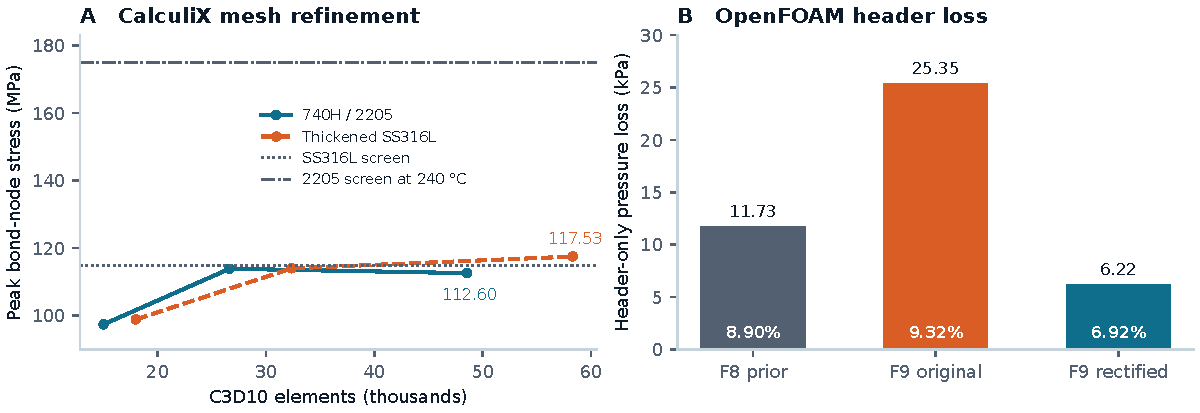
\includegraphics[width=.96\linewidth]{fig1_gate_audit.pdf}
  \caption{\textsf{MEASURED} component gate reductions. A shows the stress mesh study for 740H and Duplex 2205, which share a trace at this scale, and for thickened SS316L. B compares header-only loss with the maximum port deviation written on each bar.}
  \label{fig:gates}
\end{figure}

\subsection*{Carry-forward basis}
Keep the 740H elastic surge result and the rectified \texttt{HDR\_F9} header-only loss. Carry the archived Variant B $Nu$ and $f$ into system closure. The failure of the \texttt{RIB\_F8} friction and stationarity screens removes its thermal and pressure-drop credit.
\clearpage
% --- Section 5 ---
\section{CoolProp HEOS Closure and Economics}

Integrating the verified Gate 1--3 outcomes---full Inconel 740H recuperators, 6.222\,kPa rectified \texttt{HDR\_F9} header loss, conservative $Nu = 43.66$ ($0.59423\times$), archived friction ($0.96053\times$), \texttt{TS\_F10} (\$8.99/kWh\textsubscript{th}, 0.991 factor), commercial geared 3,600\,RPM WRSM (97.86\%, \$151/gross kW\textsubscript{e}), and \$200,000 controls---into the 192-interval CoolProp \texttt{HEOS::CO2} solver yields the rectified dry plant performance in Table~\ref{tab:heos} (pressure-closure residuals $<0.03$\,Pa).

\begin{table}[H]
  \centering
  \caption{Audited 192-interval CoolProp \texttt{HEOS::CO2} system closure for Apex-Continuum-50 v2 (Rectified Dry).}
  \label{tab:heos}
  \begin{tabularx}{\linewidth}{X r r}
    \toprule
    \textbf{System Parameter (MODELED from Continuum-Verified Inputs)} & \textbf{20\,\textdegree C ISO} & \textbf{42\,\textdegree C Summer} \\
    \midrule
    Net AC / Gross AC Export (MW) & 50.00 / 50.903 & 45.08 / 46.012 \\
    Plant CO\textsubscript{2} Mass Flow Rate (kg/s) & 307.353 & 307.353 \\
    Net AC Cycle Efficiency / AC Round-Trip Efficiency (\%) & 52.833 / \textbf{52.36} & 48.927 / \textbf{48.49} \\
    LTR Pinch / HTR Pinch Margin (K) & 10.17 / 18.660 & 11.88 / 20.153 \\
    Hottest LTR Fluid Terminal (\textdegree C) & 229.77 & 262.76 \\
    Installed Power Block CAPEX (\$M) & \textbf{65.50} & 65.50 \\
    Power Block CAPEX per Delivered Net kW\textsubscript{e} (\$/kW\textsubscript{e}) & 1,309.99 & 1,453.11 \\
    Electricity-Only 24\,h LCOS (\$/MWh) & \textbf{82.48} & \textbf{89.86} \\
    Electricity-Only 100\,h LCOS (\$/MWh) & \textbf{98.50} & \textbf{107.05} \\
    Cycle Pressure-Closure Residual (Pa) & 0.0287 & 0.0190 \\
    \bottomrule
  \end{tabularx}
\end{table}


Full 740H is retained and duplex credit is \$0. Relative to the shipped Dry claim, ISO LCOS increases by \$2.58/MWh at 24\,h and \$2.27/MWh at 100\,h (Table~\ref{tab:reconcile}). The summer point holds the ISO-sized mass flow and yields lower export on the same installed block (Figure~\ref{fig:econ}).

\begin{table}[H]
  \centering
  \caption{Zero-trust reconciliation between shipped Campaign II model and audited rectified baseline.}
  \label{tab:reconcile}
  \begin{tabularx}{\linewidth}{X r r r}
    \toprule
    \textbf{Metric} & \textbf{Shipped Dry Claim} & \textbf{Rectified Solver-Backed} & \textbf{Audit Delta} \\
    \midrule
    Installed Block CAPEX (\$M) & 58.92 & 65.50 & +6.58 \\
    ISO AC Round-Trip Efficiency (\%) & 52.44 & 52.36 & $-0.08$\,pp \\
    42\,\textdegree C Summer Net AC (MW) & 45.45 & 45.08 & $-0.37$\,MW \\
    ISO 24\,h / 100\,h LCOS (\$/MWh) & 79.90 / 96.23 & 82.48 / 98.50 & +2.58 / +2.27 \\
    42\,\textdegree C Summer 24\,h LCOS (\$/MWh) & 86.77 & 89.86 & +3.09 \\
    \bottomrule
  \end{tabularx}
\end{table}

\begin{figure}[H]
  \centering
  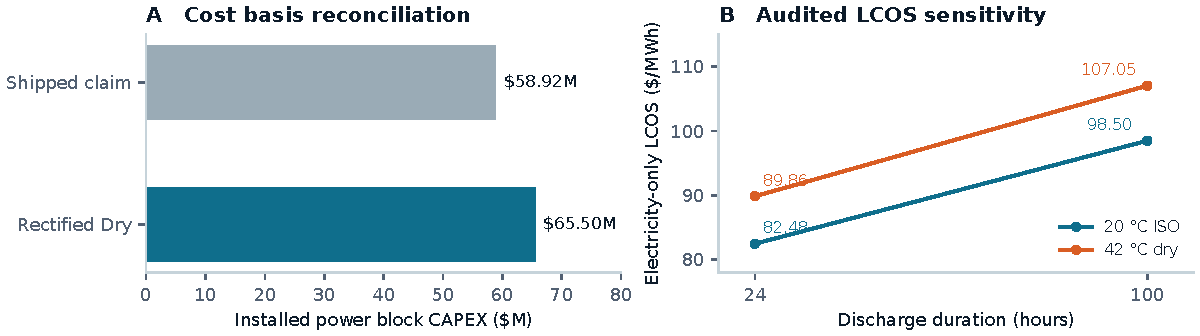
\includegraphics[width=\linewidth]{fig2_cycle_lcos.pdf}

  \caption{\textsf{MODELED} cost reconciliation and electricity-only LCOS. The historical bar is the shipped campaign premise. The rectified bar and both LCOS lines use the audited Dry case.}

  \label{fig:econ}
\end{figure}



\clearpage
% --- Section 6 ---
\section{Physical Validation and Reproducibility}\label{sec:limits}


\begin{enumerate}
  \item \textbf{740H durability.} Obtain diffusion-bond creep and fatigue coupon data. Evaluate coupled gradients and load history for code qualification.
  \item \textbf{Recuperator thermal scaling.} Extend PCHE heat-transfer validation beyond the archived periodic cell to test the module-level heat-transfer basis.
  \item \textbf{Header distribution.} Check flow uniformity on a cold-flow rig. The 6.92\% simulation result clears the fallback comparator and remains above the preferred 2.5\% target.
  \item \textbf{Vendor performance and cost.} Obtain turbomachinery maps and quotes for the geared generator train, etched 740H PCHEs and header.
  \item \textbf{Intellectual property.} Complete the \texttt{US11530625B2} claim chart for the external-plenum design \cite{us11530625}.
\end{enumerate}
The Dry cost case assigns zero credit to the duplex substitution, \texttt{RIB\_F8}, and \texttt{Desert\_Mist}. The field visualizations are numerical post-processing. The hardware items above remain open.

\begin{table}[H]
  \centering
  \caption{Cryptographic SHA-256 chain of custody for key audited artifacts (\texttt{APEX\_V2\_FINAL\_AUDIT\_REPORT.md}).}
  \label{tab:sha}
  \scriptsize\setlength{\tabcolsep}{4pt}
  \begin{tabularx}{\linewidth}{l X}
    \toprule
    \textbf{Artifact} & \textbf{SHA-256 Digest} \\
    \midrule
    \texttt{apex\_campaign\_v2\_lenovo\_handoff.zip} & \texttt{190882e4b25de9396d1132e07497cd1a36a05a09aad8ad73b3b4880cfe5a6e9b} \\
    \texttt{apex\_v2\_lenovo\_specs.json} & \texttt{4a7d625a669cfc8687b6289ff7a32219ae03a313c905e57b4a653b171e5f374d} \\
    \texttt{gate1.json} (CalculiX FEA) & \texttt{2fa31e9411845cfc40e38cb903d1fa14eba8e98bb57cfd2df9c887a6dbeebb60} \\
    \texttt{gate3\_cycle.json} (192-int.\ HEOS) & \texttt{d233a6da23fbec351ec41e531bd44de4551102c3fd92c049c555b57290e31572} \\
    \texttt{preflight.json} (2.5\,GB cap) & \texttt{61d0ebe6281d783d0bf8f36d81dd77edf3f42c98ed577b3677d0fb5021b65efc} \\
    \texttt{bond.inp} (740H mesh and load deck) & \texttt{dbb92c1fd0b236593dec7a5913038e732998daf03e494b8fb61e39254ef7146f} \\
    \texttt{bond.frd} (740H field output) & \texttt{0ce7fadcef61233d8b44213a7d6300e39021afed2b92589621e7bca7ca0d8a99} \\
    \bottomrule
  \end{tabularx}
\end{table}

% --- References ---

\begin{thebibliography}{99}\small
  \setlength{\itemsep}{2pt}
  \bibitem{audit} Apex Computational Engineering Program. \textit{Apex-Continuum-50 v2 final zero-trust continuum audit}. Project artifact \texttt{APEX\_V2\_FINAL\_AUDIT\_REPORT.md}, 25 November 2026.
  \bibitem{step_demo} GTI Energy and U.S. DOE. Supercritical Transformational Electric Power (STEP) Demo. \url{https://www.gti.energy/step-demo/}
  \bibitem{inconel740h} Special Metals. \textit{INCONEL alloy 740H technical bulletin}. \url{https://www.specialmetals.com/documents/technical-bulletins/inconel/inconel-alloy-740h.pdf}
  \bibitem{us11530625} J. O'Donnell et al. Thermal energy storage apparatus and method. U.S. Patent US11530625B2. \url{https://patents.google.com/patent/US11530625B2/en}
  \bibitem{coolprop_api} CoolProp. Low-Level API and HEOS interface. \url{https://coolprop.org/coolprop/LowLevelAPI.html}
  \bibitem{of_baffle} OpenFOAM. \texttt{porousBafflePressure} boundary condition. \url{https://doc.openfoam.com/2306/tools/processing/boundary-conditions/rtm/derived/wall/porousBafflePressure/}
  \bibitem{of_scalar} OpenFOAM v2312. \texttt{scalarTransport} source. \url{https://api.openfoam.com/2312/scalarTransport_8H_source.html}
\end{thebibliography}

\end{document}
